\begin{figure}[h]
    \centering
    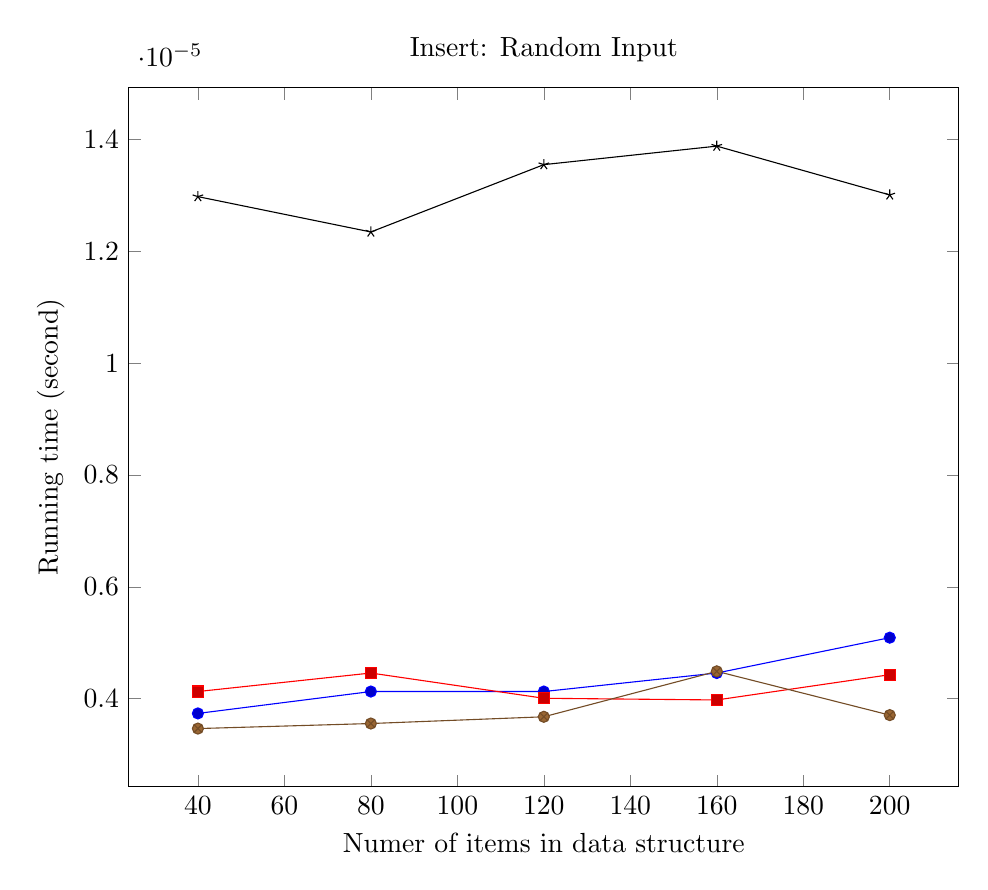
\begin{tikzpicture}
        \begin{axis}[
            xlabel={Numer of items in data structure},
            ylabel={Running time (second)},
            title={Insert: Random Input},
            width=\textwidth
        ]
		\addplot coordinates {
			(200, 5.089863191103105e-06)
			(160, 4.457394983924806e-06)
			(120, 4.1261021134976485e-06)
			(80, 4.1261021134976485e-06)
			(40, 3.73457417572054e-06)
		};
		\addplot coordinates {
			(200, 4.4272774502494835e-06)
			(160, 3.975514445121731e-06)
			(120, 4.005631978797053e-06)
			(80, 4.457394983924806e-06)
			(40, 4.1261021134976485e-06)
		};
		\addplot coordinates {
			(200, 3.7044566420459112e-06)
			(160, 4.487512517600128e-06)
			(120, 3.674339108370589e-06)
			(80, 3.5538689736699937e-06)
			(40, 3.4635163726440267e-06)
		};
		\addplot coordinates {
			(200, 1.3010774547672632e-05)
			(160, 1.3884183024252122e-05)
			(120, 1.3552890153825659e-05)
			(80, 1.2348188806818317e-05)
			(40, 1.298065701399731e-05)
		};
        \legend{}
        \end{axis}
    \end{tikzpicture}
    \caption{Average of 0 operations, benchmarked every 0, starting at 0.}
\end{figure}